\section{Eingabesprache}
Um ein zu verifizierendes GALS-Modell vollständig zu definieren müssen die folgenden Eigenschaften spezifiziert werden:
\begin{itemize}
\item Die synchronen Komponenten, aus denen das Gesamtsystem zusammen gesetzt wird.
  Jede synchrone Komponente ist eine Instanz eines in einer synchronen Sprache spezifizierten Modells.
\item Die Verbindungen zwischen den Komponenten.
  Eine Verbindung verknüpft eine Ausgabevariable einer Komponente mit einer Eingabevariable einer anderen.
\item Die zu verifizierende Eigenschaft in Form einer LTL Formel über die Variablen der einzelnen Komponenten.
\end{itemize}

\begin{figure}
  \begin{grammar}
    <declaration> ::= `model' `[' <id> `]' <id> `(' (<argument> (`,' <argument>)*)? `)' <model\_contract>
    \alt `connect' <id> `.' <id> <id> `.' <id> `;'
    \alt `verify' `{' (<formula> `;')* `}'
    
    <model\_contract> ::= `{' (<formula> `;')* `}'
    \alt `;'
    
    <formula> ::= <lit> `<' <lit>
    \alt <lit> `>' <lit>
    \alt <lit> `<=' <lit>
    \alt <lit> `>=' <lit>
    \alt <lit> `=' <lit>
    \alt <id> `in' `{' (<lit> (`,' <lit>)*)? `}'
    \alt `not' <formula>
    \alt <formula> `and' <formula>
    \alt <formula> `or' <formula>
    \alt <formula> `follows' <formula>
    \alt `always' <formula>
    \alt `next' <formula>
    \alt `(' <formula> `)'
    
    <lit> ::= <int>
    \alt <id>
    \alt <id> `.' <id>
    
    <id> ::= (`a'-`z' `A'-`Z' `0'-`9')+
    
    <int> ::= (`0'-`9')+
  \end{grammar}
  \caption{GTL Grammatik}
\end{figure}

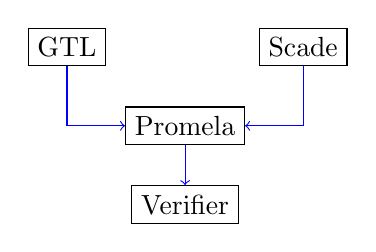
\begin{tikzpicture}
  \node[draw] (promela) at (1.5,1) {Promela};
  \node[draw] (gtl) at (0,2) {GTL};
  \node[draw] (scade) at (3,2) {Scade};
  \node[draw] (verifier) at (1.5,0) {Verifier};
  \draw[->,blue] (scade) |- (promela);
  \draw[->,blue] (gtl) |- (promela);
  \draw[->,blue] (promela) -- (verifier);
\end{tikzpicture}

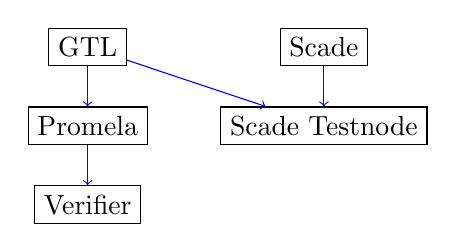
\begin{tikzpicture}
  \node[draw] (gtl) at (0,2) {GTL};
  \node[draw] (scade) at (3,2) {Scade};
  \node[draw] (promela) at (0,1) {Promela};
  \node[draw] (testnode) at (3,1) {Scade Testnode};
  \node[draw] (verifier) at (0,0) {Verifier};
  \draw[->,blue] (gtl) -- (promela);
  \draw[->,blue] (scade) -- (testnode);
  \draw[->,blue] (gtl) -- (testnode);
  \draw[->,blue] (promela) -- (verifier);
\end{tikzpicture}

